% !TeX encoding = UTF-8
\chapter{Task 4: Real-Time Classification}\label{chap:task4_realtime}

\section{Setup}\label{sec:realtime-setup}

For the real-time part, we use the binary default Decision Tree. It has the best attack F1, missed no attack on the test split, and has a false-positive rate of $18 / 48{,}611 = 0.037\,\%$. The detector loads the saved pipeline unchanged, so training and serving use exactly the same scaling, selection and classifier. Figure~\ref{fig:arch} shows the data flow. The input is the flow CSV of our own capture (Chapter~\ref{chap:task1_flows}): 569 flows produced by CICFlowMeter V4, whereas the training data comes from an older version. The detector streams the flows one by one in timestamp order, maps the V4 column names to the training names (all 77 features map), drops the \texttt{Protocol = 0} rows, replaces infinite and NaN values by 0 and classifies each flow (Listing~\ref{lst:detector}). The flow CSV is a command-line argument, so the detector can be pointed at any other V4 flow file.

\begin{figure}[ht]
	\centering
	\resizebox{\linewidth}{!}{%
	\begin{tikzpicture}[node distance=5mm, every node/.style={font=\footnotesize},
		box/.style={draw, rounded corners=2pt, align=center, minimum height=1.6cm, minimum width=2.3cm, text width=2.2cm, fill=gray!10},
		>={Stealth[length=2mm]}]
		\node[box] (a) {Capture\\\texttt{.pcapng}};
		\node[box, right=of a] (b) {CICFlowMeter\\(offline)};
		\node[box, right=of b] (c) {Flow CSV\\(V4 columns)};
		\node[box, right=of c] (d) {Column\\mapping\\V4 $\to$ training};
		\node[box, right=of d] (e) {Clean:\\drop\\\mbox{Protocol 0},\\inf/NaN $\to$ 0};
		\node[box, right=of e] (f) {Pipeline\\(scale, select,\\tree)};
		\node[box, right=of f] (g) {Verdict\\per flow};
		\foreach \x/\y in {a/b,b/c,c/d,d/e,e/f,f/g} \draw[->] (\x) -- (\y);
	\end{tikzpicture}}
	\caption{Real-time architecture. Flows are streamed row by row in timestamp order.}
	\label{fig:arch}
\end{figure}

\lstinputlisting[style=py,float=htbp,linerange={38-44,46-48,50-54,62-64,71-71},caption={Excerpt of \texttt{Detector.process()} in \texttt{src/lab2ids/realtime/detector.py}: column mapping, Protocol-0 drop, feature check, inf/NaN replacement and prediction (some lines omitted)},label={lst:detector}]{../src/lab2ids/realtime/detector.py}

\section{Correctness: Parity Test}\label{sec:parity}

To prove that the real-time path does not change the model's behavior, we converted the 49,254-flow test split to the V4 column names and streamed it through the detector. The predictions are identical, row for row, to those of the offline pipeline, both for batches of 1,000 flows and for batches of one flow. The attack F1 recomputed from the streamed predictions equals the offline value of Table~\ref{tab:t4binary}. Figure~\ref{fig:tests} shows the test evidence: 21 unit tests and 3 full-dataset tests (Task 3 numbers, Task 4 regression guards and this parity test) pass.

\begin{figure}[ht]
	\centering
	\begin{subfigure}[t]{0.45\linewidth}
		\centering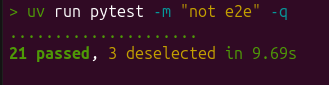
\includegraphics[width=\linewidth]{SS13.png}
		\caption{Unit tests: 21 passed.}
	\end{subfigure}\hfill
	\begin{subfigure}[t]{0.45\linewidth}
		\centering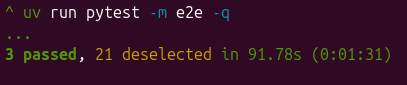
\includegraphics[width=\linewidth]{SS14.png}
		\caption{Full-dataset tests: 3 passed.}
	\end{subfigure}
	\caption{Test evidence for Tasks 3 and 4.}
	\label{fig:tests}
\end{figure}

\section{Results on Our Capture}\label{sec:realtime-results}

Of 569 flows, 22 were dropped (protocol 0) and 547 were classified: 544 as BENIGN and 3 as ATTACK, an alert rate of 0.55\,\% (Table~\ref{tab:t5rt}, Figure~\ref{fig:ss12}). Our traffic is benign by construction, so all three alerts are false positives. For the same reason, we can measure the false-positive rate on our network but not the detection rate.

\begin{table}[ht]
	\centering\small
	% AUTO-GENERATED by scripts/make_report_tables.py from outputs/realtime/run_log.txt, outputs/realtime/predictions.csv -- do not edit
\begin{tabular}{lr}
\toprule
Quantity & Value \\
\midrule
Flows read & 569 \\
Protocol-0 flows dropped & 22 \\
inf/NaN cells replaced & 0 \\
Flows classified & 547 \\
Classified BENIGN & 544 \\
ATTACK alerts & 3 \\
Alert rate & 0.55\,\% \\
Latency per flow, mean (ms) & 14.203 \\
Latency per flow, median (ms) & 13.510 \\
\bottomrule
\end{tabular}

	\caption{Real-time run on \texttt{task2\_lab2.pcap\_Flow.csv}.}
	\label{tab:t5rt}
\end{table}

\begin{figure}[ht]
	\centering
	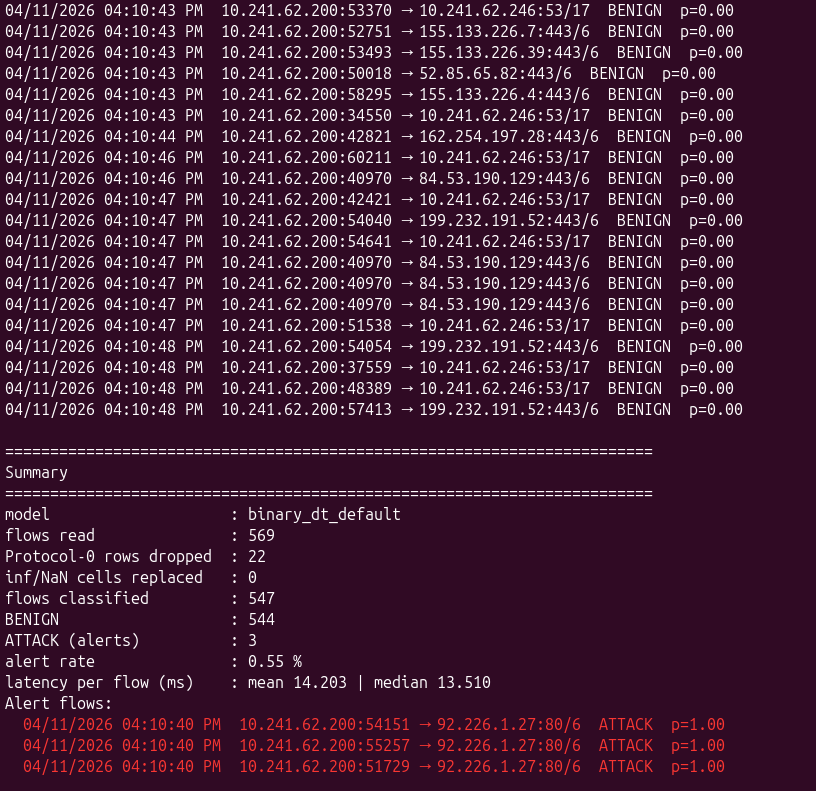
\includegraphics[width=0.7\linewidth]{SS12.png}
	\caption{Output of the real-time detector: streamed flow verdicts, the summary (569 read, 22 dropped, 547 classified, 3 alerts = 0.55\,\%) and the three alerts in red.}
	\label{fig:ss12}
\end{figure}

\section{The False Positives}\label{sec:fp}

We checked the three alerts against the capture. At 16:10:40, the Steam client sent seven parallel requests \texttt{GET /appinfo/<id>/sha/<hash>.txt.gz} over plain HTTP to \texttt{clientconfig.akamai.steamstatic.com} (\texttt{92.226.1.27:80}, Figure~\ref{fig:ss18}). All received \texttt{200 OK} with small gzip files (0.8--3.7\,kB). The seven flows are nearly identical: server initial window \texttt{Init\_Win\_bytes\_backward} = 507, client window 64,240, port 80, about 101\,ms duration and 2 PSH flags.

The tree flags them because its first splits route all seven into the region ``small server initial window ($235 < 507 \le 1{,}146$) and destination port $\le 85$''. In the training data, this region holds attacks: the Brute Force and XSS servers had small windows (235, 236 and 1,150), and every attack targets port 80. These are the shortcut features of Section~\ref{sec:t3-interp}. Only 3 of the 7 flows are flagged because the final verdict comes from a split at depth 15 on packet-length features, where the unpruned tree lets 4 near-identical flows pass and flags 3. The tree has overfitted to these fine splits.

\ssfig[0.8\linewidth]{SS18}{The seven parallel Steam requests in Wireshark (display filter at the top): \texttt{GET /appinfo/\ldots} to the Steam CDN at 92.226.1.27, all answered with \texttt{200 OK}. The host name, \texttt{clientconfig.akamai.steamstatic.com}, comes from the HTTP Host header.}{fig:ss18}

\section{Latency and Scope}\label{sec:latency}

Classifying one flow at a time takes 14.2\,ms on average (median 13.5\,ms) in our recorded run; an earlier run measured 11.6\,ms, so there is run-to-run variance. This is per-call pandas and scikit-learn overhead: batched, the same model needs 0.67\,ms per 1,000 flows. In practice, the detection delay is dominated by CICFlowMeter, which emits a flow only when it ends (FIN or RST) or times out (5\,s activity, 120\,s flow timeout). ``Real time'' here means streaming the flows of a recorded capture through the detector one by one; we do not capture packets live.

\FloatBarrier
